\chapter{Plano de cableado horizontal}
\section{Planta baja}
\begin{center}
	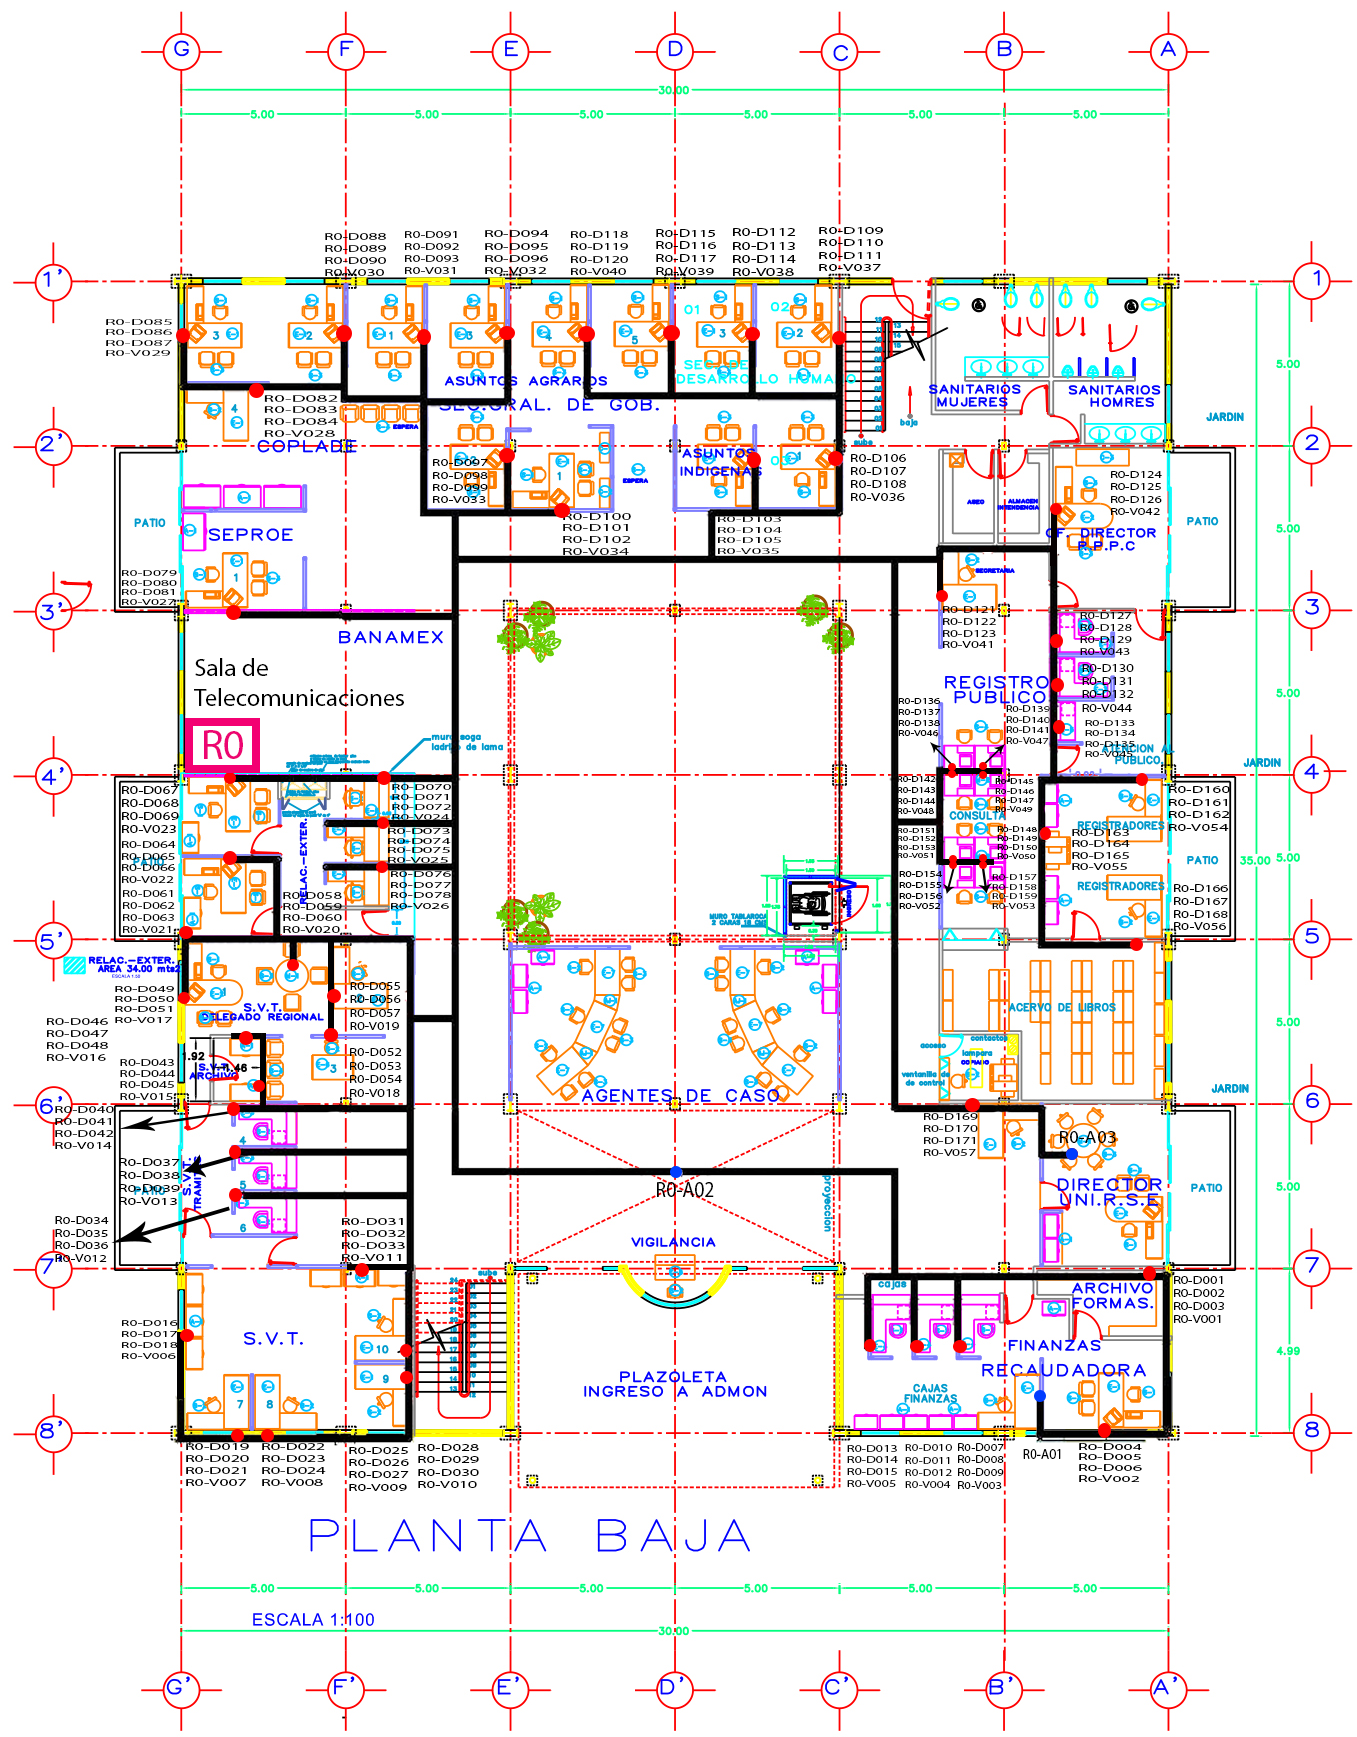
\includegraphics[scale=1.01]{CHPB.png}
\end{center}
\subsection{Salas de telecomunicaciones y de equipamiento}
La sala de telecomunicaciones y de equipamiento se encuentra en la sala nombrada como ``BANAMEX'', que es donde se encontraría el rack 0, el cual hace las funciones de rack de planta y de edificio.

\subsection{Distribuidores etiquetados}
El distribuidor de esta planta se encuentra enumerado como ``R0'' (Rack 0). Las nomenclaturas usadas en el etiquetado han seguido las siguientes normas:
\begin{itemize}
	\item \textbf{Datos. R0-DXXX:} R0 hace referencia al distribuidor de planta baja y XXX es el número de la toma de datos a la cual está conectada.
	\item \textbf{Voz. R0-VXXX:} R0 vuelve a hacer referencia al distribuidor de planta baja y XXX es el número de la toma de voz a al cual está conectada.
	\item \textbf{Puntos de acceso. R0-AXX:} R0 es de nuevo el distribuidor de planta baja y XX es el número de la toma de datos a la cual está conectado el punto de acceso.
\end{itemize}

\subsection{Tomas de comunicaciones etiquetadas instaladas en cada sala}
En cuanto a las tomas de comunicaciones de esta planta, encontramos 171 tomas de datos, 57 tomas de voz y 3 puntos de acceso distribuidos por toda la planta baja.

\newpage
\section{Planta alta}
\begin{center}
	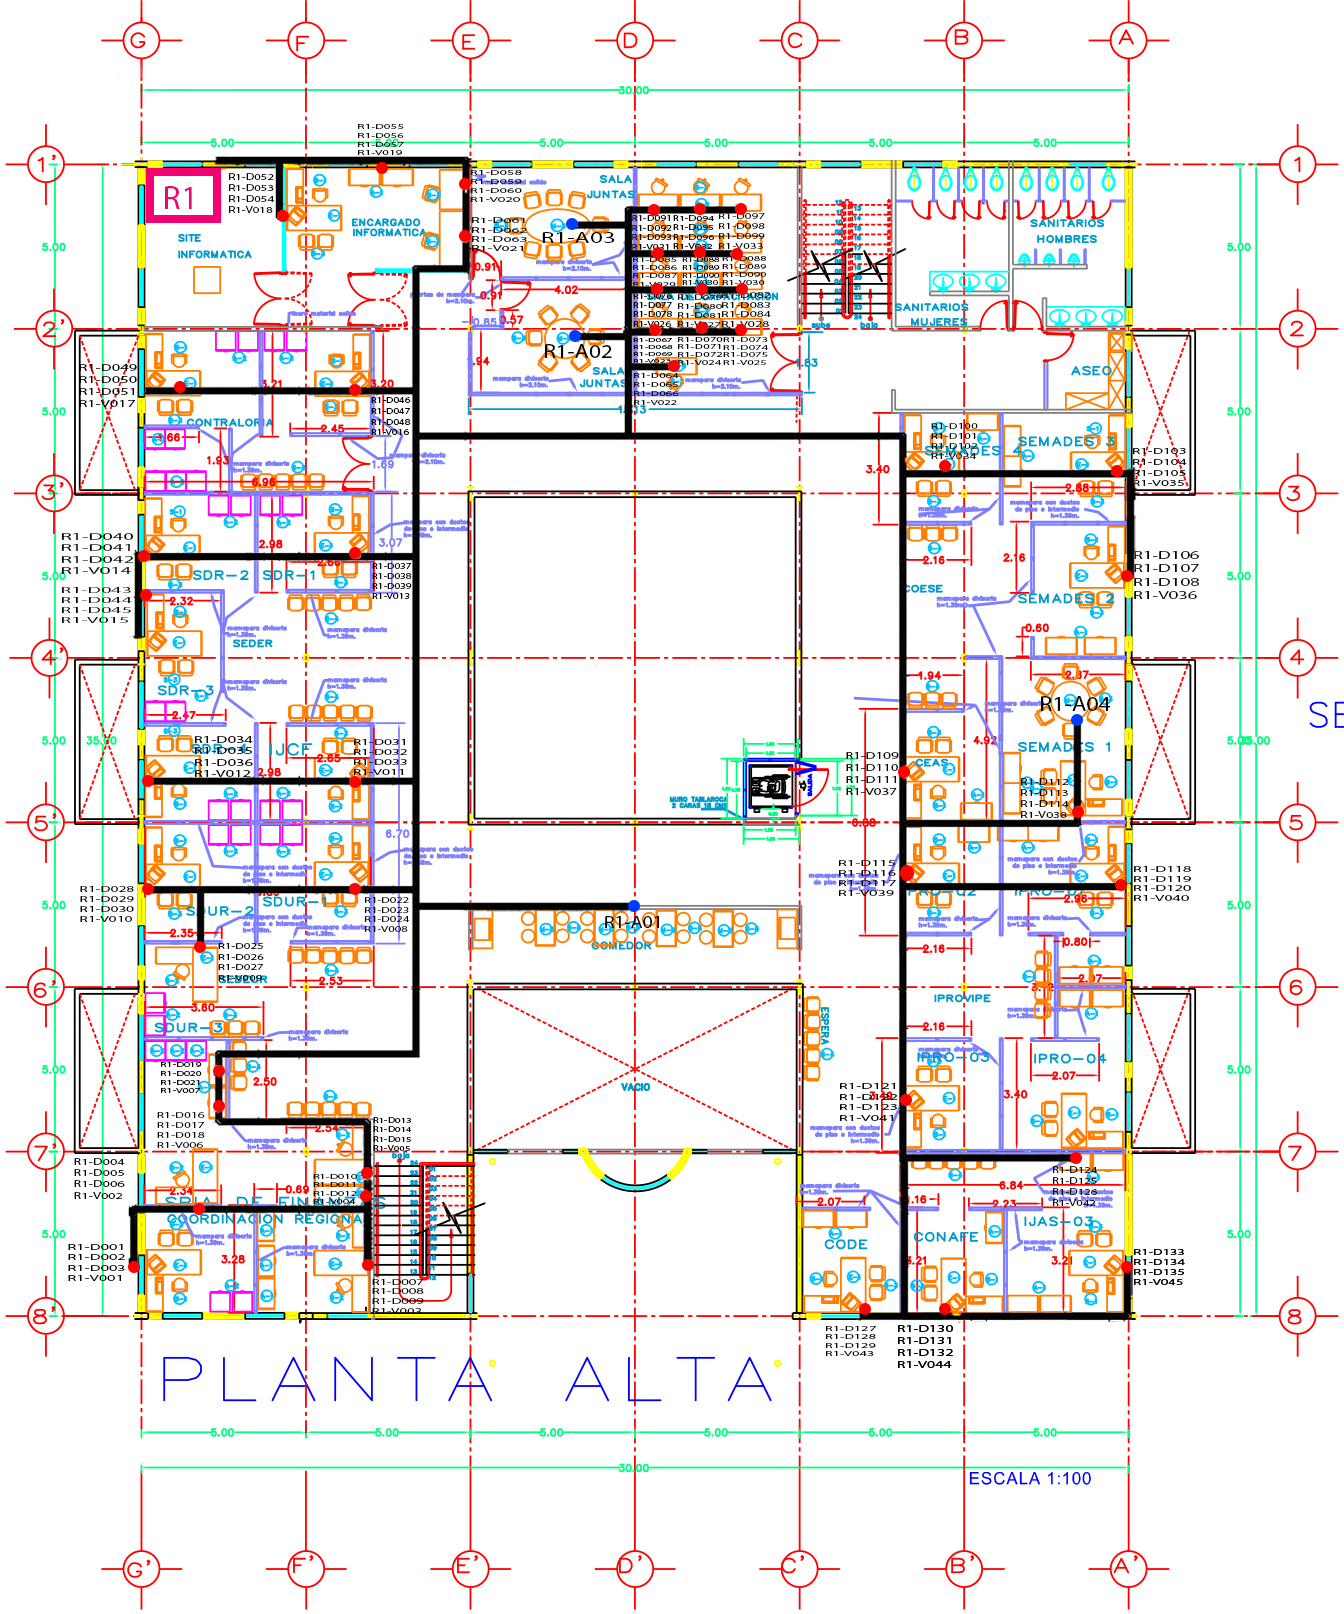
\includegraphics[scale=1.3]{CHPA.png}
\end{center}
\subsection{Salas de telecomunicaciones y de equipamiento}
La sala de telecomunicaciones y de equipamiento se encuentra en la sala nombrada como ``SITE INFORMÁTICA'' que es donde se encontraría el rack 1, el cual hace la función de rack de planta.

\subsection{Distribuidores etiquetados}
El distribuidor de esta planta se encuentra enumerado como ``R1'' (Rack 1). Las nomenclaturas usadas en el etiquetado han seguido las mismas normas que en la planta baja.

\subsection{Tomas de comunicaciones etiquetadas instaladas en cada sala}
En cuanto a las tomas de comunicaciones de esta planta, encontramos 135 tomas de datos, 45 tomas de voz y 4 puntos de acceso distribuidos por toda la planta alta.
